\chapter{绪\hspace{6pt}论}

\section{研究工作的背景与意义}
\subsection{研究背景}

随着信息技术产业的高速发展,数字信息量呈爆炸式增长。Gartner研究表明\citing{gartner2015} ,仅2015年的移动数据流量就较2014年增长59\%;并且,这一增长率将持至2018年末,移动数据流量水平达1.73亿TB。数据的快速增长导致企业面临的存储和管理成本越来越高\citing{敖莉2010重复数据删除技术}。另一方面,在存储系统所保存的数据中,高达60\%的数据都是冗余的,随着时间的推移,这些冗余数据的比例将进一步上升\citing{mcknight2006digital}。近年来,存储系统中数据高冗余的特点得到越来越多研究人员的关注,利用该特点来节省存储容量是一个热门研究课题。

重复数据删除技术(data deduplication)是指通过识别数据流中的冗余,只传输或存储唯一数据(unique data),而使用指向已存储数据的指针替换重复副本, 以达到节省带宽或存储空间的目的\citing{2012重复数据删除关键技术研究进展}。由于能够有效地降低存储开销,重复数据删除技术非常适合为管理日益增长的海量数据节省成本。在工业界,EMC Data Domain\citing{EMCDataDomain}和Avamar\citing{Avamar}、Veritas的NetBackup Appliances\citing{veritas} 以及Commvault的开放数据平台\citing{CommVault} 都是比较知名的数据重删应用产品;此外,各大云存储厂商(例如 Dropbox、Google Drive、Bitcasa、Moza等)也纷纷将重复数据删除技术应用于各自的云服务产品中,以提升经济效益\citing{harnik2010side}。

如图\ref{fig:数据重删系统的存储模式}所示,在支持数据重删的存储系统(统称为数据重删系统)中,重删后的任何数据块都被一个或多个文件引用,而文件则以指向这些数据块的指针的集合形式存储。这种文件共用数据块的存储模式强调了数据块的敏感性,因为一个数据块的泄漏可能扩散影响到共用这个数据块的所有文件。如何保护重删后的数据的隐私,成为信息安全领域的一个研究热点。

\begin{figure}[!htb]
    \small
    \centering
    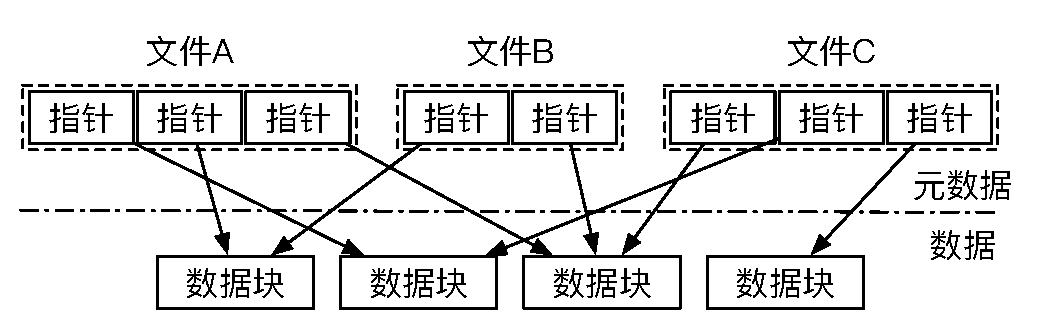
\includegraphics[width=10cm]{DedupSystemStorageMode.eps}
    \caption{数据重删系统的存储模式} 
    \label{fig:数据重删系统的存储模式}
\end{figure}

为了保护数据隐私,加密重复数据删除(encrypted deduplication)增加了一层作用于逻辑数据块的加密操作。如图\ref{fig:加密重复数据删除系统逻辑视图}所示,该加密层基于数据内容来产生加密密钥\citing{bellare2013message}(例如将数据块的哈希值作为密钥\citing{douceur2002reclaiming}),从而将相同的明文数据块加密为相同的密文数据块。系统计算每个密文数据块的哈希值(称为指纹,fingerprint),查询指纹索引(fingerprint index)确定该数据块是否已经存储,最后保存仅具有唯一指纹的密文数据块。需要指出的是,部分加密重复数据删除方案\citing{bellare2013message}采用随机加密算法,但基于明文数据块产生指纹,因此仍然可以通过检查指纹来识别重复数据。

\begin{figure}[!htb]
    \small
    \centering
    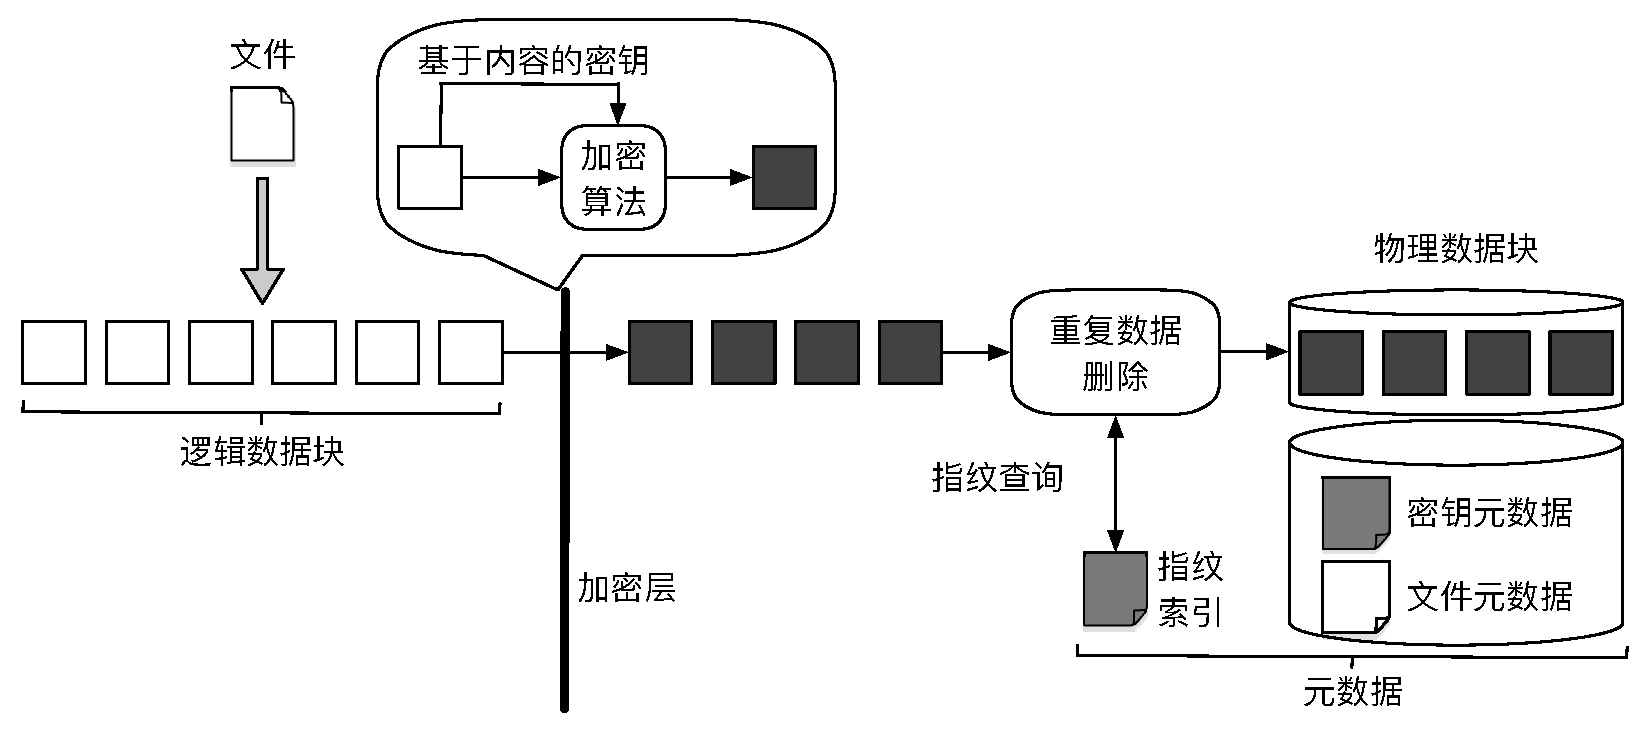
\includegraphics[width=14cm]{EncryptDedupSystemLogic.eps}
    \caption{加密重复数据删除系统逻辑视图}
    \label{fig:加密重复数据删除系统逻辑视图}
\end{figure}

消息锁定加密(MLE)将加密原语形式化,用于加密重复数据删除。它指定了对称密钥(成为MLE密钥)如何从明文数据块的内容


% 消息锁定加密 (MLE) \citing{bellare13a} 将加密原语形式化,用于加密重复数据删除。它指定了对称密钥(称为 MLE 密钥)如何从明文块的 内容(例如,其流行的实例化收敛加密(CE) \citing{douceur02}使用明文块的加密哈希作为 MLE 密钥)。因此,它将重复的明文块加密为重复的密文块,以便重复数据删除在密文块上仍然可行。

% \paragraph{Server-aided MLE.} CE 容易受到{\em 离线暴力攻击},因为它的 MLE 密钥(即明文块的哈希)可以公开导出。具体来说,对手通过枚举所有可能的明文块的 MLE 密钥来从目标密文块(不知道 MLE 密钥)推断输入明文块,以检查是否有任何明文块被加密为目标密文块。

% 服务器辅助 MLE \citing{bellare13b} 是一种最先进的加密原语,可增强加密重复数据删除的安全性,防止离线暴力攻击。

% 它为 MLE 密钥生成部署了一个专用的 {\em 密钥服务器}。为了加密明文块,客户端首先将明文块的指纹发送到密钥服务器,密钥服务器通过指纹和密钥服务器维护的 {\em global secret} 返回 MLE 密钥。如果全局秘密是安全的,对手就不可能发起离线暴力攻击;否则,如果全局秘密被泄露,安全性将降低到原始 MLE 的安全性。服务器辅助 MLE 进一步建立在两个安全机制之上。首先,它使用 {\em 遗忘伪随机函数 (OPRF)} \citing{naor04} 来允许客户端发送明文块的“盲”指纹,这样密钥服务器仍然可以返回相同的 MLE 密钥以获得相同的指纹无需学习原始指纹。其次,它对来自客户端的密钥生成请求进行速率限制以防止{\em 在线暴力攻击},其中恶意客户端向密钥服务器发出许多密钥生成请求,以便找到目标 MLE 密钥。

% \paragraph{所有权证明。}为了节省带宽,加密重复数据删除可以应用基于源的重复数据删除,而不是基于目标的重复数据删除,以在客户端删除重复的密文块,而无需上传到云端(\S)。客户端将密文块的指纹发送到云端,云端检查指纹是否被指纹索引跟踪(即,对应的密文块已经存储)。然后客户端仅将非重复的密文块上传到云。 







\subsection{问题和动机}
\subsection{研究意义}





\citing{ren2021accelerating}
\section{国内外研究历史与现状}

\subsection{加密重复数据删除}
\subsubsection{加密重复数据删除技术}
\subsubsection{服务器辅助密钥生成}
\subsubsection{所有权证明技术}
\subsection{可信计算平台}
\subsubsection{Intel SGX}
\subsubsection{AMD SEV}
\subsubsection{ARM Trusted Zone}


\section{本文的主要贡献与创新}

\section{本论文的结构安排}